\documentclass{standalone}
\usepackage{tikz}
\usetikzlibrary{patterns, positioning}


\begin{document}
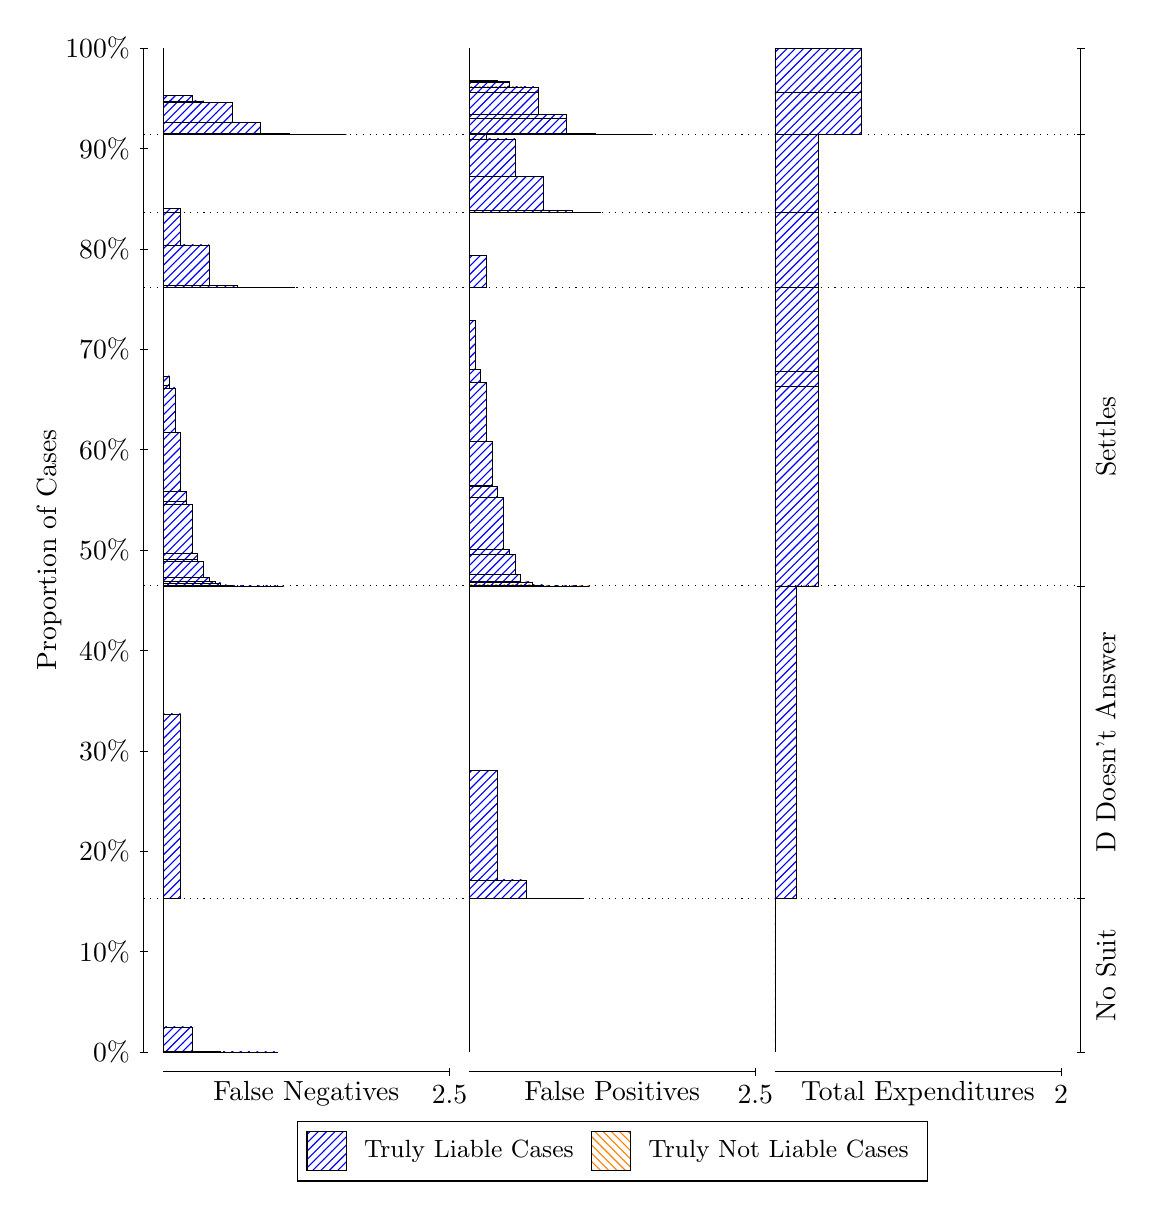
\begin{tikzpicture}
\draw[black, very thin] (1.5,1.75) -- (1.5,14.5);
\node[rotate=90, text=black, anchor=center] at (0.3, 8.125) {Proportion of Cases};
\draw[black, very thin] (1.45,1.75) -- (1.55,1.75);
\node[text=black, anchor=east] at (1.45, 1.75) {0\%};
\draw[black, very thin] (1.45,3.025) -- (1.55,3.025);
\node[text=black, anchor=east] at (1.45, 3.025) {10\%};
\draw[black, very thin] (1.45,4.3) -- (1.55,4.3);
\node[text=black, anchor=east] at (1.45, 4.3) {20\%};
\draw[black, very thin] (1.45,5.575) -- (1.55,5.575);
\node[text=black, anchor=east] at (1.45, 5.575) {30\%};
\draw[black, very thin] (1.45,6.85) -- (1.55,6.85);
\node[text=black, anchor=east] at (1.45, 6.85) {40\%};
\draw[black, very thin] (1.45,8.125) -- (1.55,8.125);
\node[text=black, anchor=east] at (1.45, 8.125) {50\%};
\draw[black, very thin] (1.45,9.4) -- (1.55,9.4);
\node[text=black, anchor=east] at (1.45, 9.4) {60\%};
\draw[black, very thin] (1.45,10.675) -- (1.55,10.675);
\node[text=black, anchor=east] at (1.45, 10.675) {70\%};
\draw[black, very thin] (1.45,11.95) -- (1.55,11.95);
\node[text=black, anchor=east] at (1.45, 11.95) {80\%};
\draw[black, very thin] (1.45,13.225) -- (1.55,13.225);
\node[text=black, anchor=east] at (1.45, 13.225) {90\%};
\draw[black, very thin] (1.45,14.5) -- (1.55,14.5);
\node[text=black, anchor=east] at (1.45, 14.5) {100\%};

\draw[black, very thin] (13.4,1.75) -- (13.4,14.5);
\draw[black, very thin] (13.35,1.75) -- (13.45,1.75);
\node[anchor=west] at (13.35, 1.75) {};
\draw[black, very thin] (13.35,3.7026) -- (13.45,3.7026);
\node[anchor=west] at (13.35, 3.7026) {};
\draw[black, very thin] (13.35,7.6689) -- (13.45,7.6689);
\node[anchor=west] at (13.35, 7.6689) {};
\draw[black, very thin] (13.35,11.456) -- (13.45,11.456);
\node[anchor=west] at (13.35, 11.456) {};
\draw[black, very thin] (13.35,12.411) -- (13.45,12.411);
\node[anchor=west] at (13.35, 12.411) {};
\draw[black, very thin] (13.35,13.401) -- (13.45,13.401);
\node[anchor=west] at (13.35, 13.401) {};
\draw[black, very thin] (13.35,14.5) -- (13.45,14.5);
\node[anchor=west] at (13.35, 14.5) {};

\draw[black, very thin, pattern color=blue, pattern=north east lines] (1.75,1.75) rectangle (3.2033,1.75);
\draw[black, very thin, pattern color=blue, pattern=north east lines] (1.75,1.75) rectangle (2.84,1.75);
\draw[black, very thin, pattern color=blue, pattern=north east lines] (1.75,1.75) rectangle (2.4767,1.7527);
\draw[black, very thin, pattern color=blue, pattern=north east lines] (1.75,1.7527) rectangle (2.1133,2.0697);
\draw[black, very thin, pattern color=orange, pattern=north west lines] (1.75,2.0697) rectangle (1.75,2.0697);
\draw[black, very thin, pattern color=blue, pattern=north east lines] (1.75,2.0697) rectangle (1.75,3.7026);
\draw[black, very thin, pattern color=blue, pattern=north east lines] (1.75,3.7026) rectangle (1.968,6.0428);
\draw[black, very thin, pattern color=orange, pattern=north west lines] (1.75,6.0428) rectangle (1.75,6.0428);
\draw[black, very thin, pattern color=blue, pattern=north east lines] (1.75,6.0428) rectangle (1.75,7.6689);
\draw[black, very thin, pattern color=blue, pattern=north east lines] (1.75,7.6689) rectangle (3.276,7.6689);
\draw[black, very thin, pattern color=blue, pattern=north east lines] (1.75,7.6689) rectangle (3.1307,7.6689);
\draw[black, very thin, pattern color=blue, pattern=north east lines] (1.75,7.6689) rectangle (2.9853,7.6689);
\draw[black, very thin, pattern color=blue, pattern=north east lines] (1.75,7.6689) rectangle (2.9127,7.6689);
\draw[black, very thin, pattern color=blue, pattern=north east lines] (1.75,7.6689) rectangle (2.84,7.6689);
\draw[black, very thin, pattern color=blue, pattern=north east lines] (1.75,7.6689) rectangle (2.7673,7.669);
\draw[black, very thin, pattern color=blue, pattern=north east lines] (1.75,7.669) rectangle (2.6947,7.669);
\draw[black, very thin, pattern color=blue, pattern=north east lines] (1.75,7.669) rectangle (2.622,7.6791);
\draw[black, very thin, pattern color=blue, pattern=north east lines] (1.75,7.6791) rectangle (2.5493,7.6814);
\draw[black, very thin, pattern color=blue, pattern=north east lines] (1.75,7.6814) rectangle (2.4767,7.7076);
\draw[black, very thin, pattern color=blue, pattern=north east lines] (1.75,7.7076) rectangle (2.404,7.7079);
\draw[black, very thin, pattern color=blue, pattern=north east lines] (1.75,7.7079) rectangle (2.404,7.7223);
\draw[black, very thin, pattern color=blue, pattern=north east lines] (1.75,7.7223) rectangle (2.3313,7.7723);
\draw[black, very thin, pattern color=blue, pattern=north east lines] (1.75,7.7723) rectangle (2.2587,7.9823);
\draw[black, very thin, pattern color=blue, pattern=north east lines] (1.75,7.9823) rectangle (2.186,8.0106);
\draw[black, very thin, pattern color=blue, pattern=north east lines] (1.75,8.0106) rectangle (2.186,8.083);
\draw[black, very thin, pattern color=blue, pattern=north east lines] (1.75,8.083) rectangle (2.1133,8.7058);
\draw[black, very thin, pattern color=blue, pattern=north east lines] (1.75,8.7058) rectangle (2.0407,8.7376);
\draw[black, very thin, pattern color=blue, pattern=north east lines] (1.75,8.7376) rectangle (2.0407,8.8731);
\draw[black, very thin, pattern color=blue, pattern=north east lines] (1.75,8.8731) rectangle (1.968,9.6196);
\draw[black, very thin, pattern color=blue, pattern=north east lines] (1.75,9.6196) rectangle (1.8953,10.177);
\draw[black, very thin, pattern color=blue, pattern=north east lines] (1.75,10.177) rectangle (1.8953,10.185);
\draw[black, very thin, pattern color=blue, pattern=north east lines] (1.75,10.185) rectangle (1.8227,10.22);
\draw[black, very thin, pattern color=blue, pattern=north east lines] (1.75,10.22) rectangle (1.8227,10.336);
\draw[black, very thin, pattern color=blue, pattern=north east lines] (1.75,10.336) rectangle (1.75,10.336);
\draw[black, very thin, pattern color=orange, pattern=north west lines] (1.75,10.336) rectangle (1.75,10.336);
\draw[black, very thin, pattern color=blue, pattern=north east lines] (1.75,10.336) rectangle (1.75,11.456);
\draw[black, very thin, pattern color=blue, pattern=north east lines] (1.75,11.456) rectangle (3.4213,11.456);
\draw[black, very thin, pattern color=blue, pattern=north east lines] (1.75,11.456) rectangle (3.058,11.456);
\draw[black, very thin, pattern color=blue, pattern=north east lines] (1.75,11.456) rectangle (2.6947,11.489);
\draw[black, very thin, pattern color=blue, pattern=north east lines] (1.75,11.489) rectangle (2.3313,12.001);
\draw[black, very thin, pattern color=blue, pattern=north east lines] (1.75,12.001) rectangle (1.968,12.411);
\draw[black, very thin, pattern color=orange, pattern=north west lines] (1.75,12.411) rectangle (1.75,12.411);
\draw[black, very thin, pattern color=blue, pattern=north east lines] (1.75,12.411) rectangle (1.968,12.465);
\draw[black, very thin, pattern color=orange, pattern=north west lines] (1.75,12.465) rectangle (1.75,12.465);
\draw[black, very thin, pattern color=blue, pattern=north east lines] (1.75,12.465) rectangle (1.75,13.401);
\draw[black, very thin, pattern color=blue, pattern=north east lines] (1.75,13.401) rectangle (4.0753,13.401);
\draw[black, very thin, pattern color=blue, pattern=north east lines] (1.75,13.401) rectangle (3.712,13.401);
\draw[black, very thin, pattern color=blue, pattern=north east lines] (1.75,13.401) rectangle (3.3487,13.413);
\draw[black, very thin, pattern color=blue, pattern=north east lines] (1.75,13.413) rectangle (2.9853,13.559);
\draw[black, very thin, pattern color=blue, pattern=north east lines] (1.75,13.559) rectangle (2.84,13.559);
\draw[black, very thin, pattern color=blue, pattern=north east lines] (1.75,13.559) rectangle (2.622,13.811);
\draw[black, very thin, pattern color=blue, pattern=north east lines] (1.75,13.811) rectangle (2.4767,13.814);
\draw[black, very thin, pattern color=blue, pattern=north east lines] (1.75,13.814) rectangle (2.2587,13.83);
\draw[black, very thin, pattern color=blue, pattern=north east lines] (1.75,13.83) rectangle (2.1133,13.895);
\draw[black, very thin, pattern color=blue, pattern=north east lines] (1.75,13.895) rectangle (1.8953,13.895);
\draw[black, very thin, pattern color=orange, pattern=north west lines] (1.75,13.895) rectangle (1.75,13.895);
\draw[black, very thin, pattern color=blue, pattern=north east lines] (1.75,13.895) rectangle (1.75,14.5);
\draw[black, very thin, pattern color=orange, pattern=north west lines] (5.6333,1.75) rectangle (5.6333,1.75);
\draw[black, very thin, pattern color=blue, pattern=north east lines] (5.6333,1.75) rectangle (5.6333,3.7026);
\draw[black, very thin, pattern color=orange, pattern=north west lines] (5.6333,3.7026) rectangle (7.0867,3.7026);
\draw[black, very thin, pattern color=blue, pattern=north east lines] (5.6333,3.7026) rectangle (7.0867,3.7026);
\draw[black, very thin, pattern color=blue, pattern=north east lines] (5.6333,3.7026) rectangle (6.7233,3.7044);
\draw[black, very thin, pattern color=blue, pattern=north east lines] (5.6333,3.7044) rectangle (6.36,3.9357);
\draw[black, very thin, pattern color=blue, pattern=north east lines] (5.6333,3.9357) rectangle (5.9967,5.3287);
\draw[black, very thin, pattern color=blue, pattern=north east lines] (5.6333,5.3287) rectangle (5.6333,7.6689);
\draw[black, very thin, pattern color=orange, pattern=north west lines] (5.6333,7.6689) rectangle (7.1593,7.6689);
\draw[black, very thin, pattern color=blue, pattern=north east lines] (5.6333,7.6689) rectangle (7.1593,7.6689);
\draw[black, very thin, pattern color=orange, pattern=north west lines] (5.6333,7.6689) rectangle (7.014,7.6689);
\draw[black, very thin, pattern color=blue, pattern=north east lines] (5.6333,7.6689) rectangle (7.014,7.6689);
\draw[black, very thin, pattern color=orange, pattern=north west lines] (5.6333,7.6689) rectangle (6.8687,7.6689);
\draw[black, very thin, pattern color=blue, pattern=north east lines] (5.6333,7.6689) rectangle (6.8687,7.6689);
\draw[black, very thin, pattern color=blue, pattern=north east lines] (5.6333,7.6689) rectangle (6.796,7.6689);
\draw[black, very thin, pattern color=orange, pattern=north west lines] (5.6333,7.6689) rectangle (6.7233,7.6689);
\draw[black, very thin, pattern color=blue, pattern=north east lines] (5.6333,7.6689) rectangle (6.7233,7.6689);
\draw[black, very thin, pattern color=blue, pattern=north east lines] (5.6333,7.6689) rectangle (6.6507,7.6689);
\draw[black, very thin, pattern color=orange, pattern=north west lines] (5.6333,7.6689) rectangle (6.578,7.6689);
\draw[black, very thin, pattern color=blue, pattern=north east lines] (5.6333,7.6689) rectangle (6.578,7.6819);
\draw[black, very thin, pattern color=blue, pattern=north east lines] (5.6333,7.6819) rectangle (6.5053,7.6821);
\draw[black, very thin, pattern color=orange, pattern=north west lines] (5.6333,7.6821) rectangle (6.4327,7.6821);
\draw[black, very thin, pattern color=blue, pattern=north east lines] (5.6333,7.6821) rectangle (6.4327,7.7201);
\draw[black, very thin, pattern color=orange, pattern=north west lines] (5.6333,7.7201) rectangle (6.4327,7.7201);
\draw[black, very thin, pattern color=blue, pattern=north east lines] (5.6333,7.7201) rectangle (6.4327,7.7201);
\draw[black, very thin, pattern color=blue, pattern=north east lines] (5.6333,7.7201) rectangle (6.36,7.7204);
\draw[black, very thin, pattern color=blue, pattern=north east lines] (5.6333,7.7204) rectangle (6.2873,7.722);
\draw[black, very thin, pattern color=orange, pattern=north west lines] (5.6333,7.722) rectangle (6.2873,7.722);
\draw[black, very thin, pattern color=blue, pattern=north east lines] (5.6333,7.722) rectangle (6.2873,7.8174);
\draw[black, very thin, pattern color=blue, pattern=north east lines] (5.6333,7.8174) rectangle (6.2147,8.0652);
\draw[black, very thin, pattern color=orange, pattern=north west lines] (5.6333,8.0652) rectangle (6.142,8.0652);
\draw[black, very thin, pattern color=blue, pattern=north east lines] (5.6333,8.0652) rectangle (6.142,8.1339);
\draw[black, very thin, pattern color=blue, pattern=north east lines] (5.6333,8.1339) rectangle (6.0693,8.7888);
\draw[black, very thin, pattern color=blue, pattern=north east lines] (5.6333,8.7888) rectangle (6.0693,8.7888);
\draw[black, very thin, pattern color=orange, pattern=north west lines] (5.6333,8.7888) rectangle (5.9967,8.7888);
\draw[black, very thin, pattern color=blue, pattern=north east lines] (5.6333,8.7888) rectangle (5.9967,8.9401);
\draw[black, very thin, pattern color=blue, pattern=north east lines] (5.6333,8.9401) rectangle (5.924,8.9484);
\draw[black, very thin, pattern color=blue, pattern=north east lines] (5.6333,8.9484) rectangle (5.924,9.5056);
\draw[black, very thin, pattern color=blue, pattern=north east lines] (5.6333,9.5056) rectangle (5.8513,10.252);
\draw[black, very thin, pattern color=blue, pattern=north east lines] (5.6333,10.252) rectangle (5.7787,10.419);
\draw[black, very thin, pattern color=blue, pattern=north east lines] (5.6333,10.419) rectangle (5.706,11.041);
\draw[black, very thin, pattern color=blue, pattern=north east lines] (5.6333,11.041) rectangle (5.706,11.042);
\draw[black, very thin, pattern color=blue, pattern=north east lines] (5.6333,11.042) rectangle (5.6333,11.456);
\draw[black, very thin, pattern color=orange, pattern=north west lines] (5.6333,11.456) rectangle (5.8513,11.456);
\draw[black, very thin, pattern color=blue, pattern=north east lines] (5.6333,11.456) rectangle (5.8513,11.866);
\draw[black, very thin, pattern color=blue, pattern=north east lines] (5.6333,11.866) rectangle (5.6333,12.411);
\draw[black, very thin, pattern color=orange, pattern=north west lines] (5.6333,12.411) rectangle (7.3047,12.411);
\draw[black, very thin, pattern color=blue, pattern=north east lines] (5.6333,12.411) rectangle (7.3047,12.411);
\draw[black, very thin, pattern color=blue, pattern=north east lines] (5.6333,12.411) rectangle (6.9413,12.44);
\draw[black, very thin, pattern color=blue, pattern=north east lines] (5.6333,12.44) rectangle (6.578,12.871);
\draw[black, very thin, pattern color=blue, pattern=north east lines] (5.6333,12.871) rectangle (6.2147,13.347);
\draw[black, very thin, pattern color=blue, pattern=north east lines] (5.6333,13.347) rectangle (5.8513,13.401);
\draw[black, very thin, pattern color=orange, pattern=north west lines] (5.6333,13.401) rectangle (7.9587,13.401);
\draw[black, very thin, pattern color=blue, pattern=north east lines] (5.6333,13.401) rectangle (7.9587,13.401);
\draw[black, very thin, pattern color=orange, pattern=north west lines] (5.6333,13.401) rectangle (7.5953,13.401);
\draw[black, very thin, pattern color=blue, pattern=north east lines] (5.6333,13.401) rectangle (7.5953,13.401);
\draw[black, very thin, pattern color=orange, pattern=north west lines] (5.6333,13.401) rectangle (7.232,13.401);
\draw[black, very thin, pattern color=blue, pattern=north east lines] (5.6333,13.401) rectangle (7.232,13.42);
\draw[black, very thin, pattern color=blue, pattern=north east lines] (5.6333,13.42) rectangle (6.8687,13.604);
\draw[black, very thin, pattern color=orange, pattern=north west lines] (5.6333,13.604) rectangle (6.8687,13.604);
\draw[black, very thin, pattern color=blue, pattern=north east lines] (5.6333,13.604) rectangle (6.8687,13.659);
\draw[black, very thin, pattern color=blue, pattern=north east lines] (5.6333,13.659) rectangle (6.5053,13.943);
\draw[black, very thin, pattern color=blue, pattern=north east lines] (5.6333,13.943) rectangle (6.5053,14.006);
\draw[black, very thin, pattern color=orange, pattern=north west lines] (5.6333,14.006) rectangle (6.36,14.006);
\draw[black, very thin, pattern color=blue, pattern=north east lines] (5.6333,14.006) rectangle (6.36,14.006);
\draw[black, very thin, pattern color=blue, pattern=north east lines] (5.6333,14.006) rectangle (6.142,14.059);
\draw[black, very thin, pattern color=blue, pattern=north east lines] (5.6333,14.059) rectangle (6.142,14.072);
\draw[black, very thin, pattern color=orange, pattern=north west lines] (5.6333,14.072) rectangle (5.9967,14.072);
\draw[black, very thin, pattern color=blue, pattern=north east lines] (5.6333,14.072) rectangle (5.9967,14.088);
\draw[black, very thin, pattern color=blue, pattern=north east lines] (5.6333,14.088) rectangle (5.7787,14.089);
\draw[black, very thin, pattern color=blue, pattern=north east lines] (5.6333,14.089) rectangle (5.7787,14.09);
\draw[black, very thin, pattern color=orange, pattern=north west lines] (5.6333,14.09) rectangle (5.6333,14.09);
\draw[black, very thin, pattern color=blue, pattern=north east lines] (5.6333,14.09) rectangle (5.6333,14.5);
\draw[black, very thin, pattern color=orange, pattern=north west lines] (9.5167,1.75) rectangle (9.5167,1.75);
\draw[black, very thin, pattern color=blue, pattern=north east lines] (9.5167,1.75) rectangle (9.5167,3.7026);
\draw[black, very thin, pattern color=orange, pattern=north west lines] (9.5167,3.7026) rectangle (9.7892,3.7026);
\draw[black, very thin, pattern color=blue, pattern=north east lines] (9.5167,3.7026) rectangle (9.7892,7.6689);
\draw[black, very thin, pattern color=orange, pattern=north west lines] (9.5167,7.6689) rectangle (10.062,7.6689);
\draw[black, very thin, pattern color=blue, pattern=north east lines] (9.5167,7.6689) rectangle (10.062,10.205);
\draw[black, very thin, pattern color=orange, pattern=north west lines] (9.5167,10.205) rectangle (10.062,10.205);
\draw[black, very thin, pattern color=blue, pattern=north east lines] (9.5167,10.205) rectangle (10.062,10.396);
\draw[black, very thin, pattern color=orange, pattern=north west lines] (9.5167,10.396) rectangle (10.062,10.396);
\draw[black, very thin, pattern color=blue, pattern=north east lines] (9.5167,10.396) rectangle (10.062,11.456);
\draw[black, very thin, pattern color=orange, pattern=north west lines] (9.5167,11.456) rectangle (10.062,11.456);
\draw[black, very thin, pattern color=blue, pattern=north east lines] (9.5167,11.456) rectangle (10.062,12.411);
\draw[black, very thin, pattern color=orange, pattern=north west lines] (9.5167,12.411) rectangle (10.062,12.411);
\draw[black, very thin, pattern color=blue, pattern=north east lines] (9.5167,12.411) rectangle (10.062,13.401);
\draw[black, very thin, pattern color=orange, pattern=north west lines] (9.5167,13.401) rectangle (10.607,13.401);
\draw[black, very thin, pattern color=blue, pattern=north east lines] (9.5167,13.401) rectangle (10.607,13.941);
\draw[black, very thin, pattern color=orange, pattern=north west lines] (9.5167,13.941) rectangle (10.607,13.941);
\draw[black, very thin, pattern color=blue, pattern=north east lines] (9.5167,13.941) rectangle (10.607,14.5);
\draw[black, dotted] (1.5,3.7026) -- (13.4,3.7026);
\draw[black, dotted] (1.5,7.6689) -- (13.4,7.6689);
\draw[black, dotted] (1.5,11.456) -- (13.4,11.456);
\draw[black, dotted] (1.5,12.411) -- (13.4,12.411);
\draw[black, dotted] (1.5,13.401) -- (13.4,13.401);
\draw[black, very thin] (1.75,1.5) -- (5.3833,1.5);
\node[text=black, anchor=north] at (3.5667, 1.5) {False Negatives};
\draw[black, very thin] (5.3833,1.45) -- (5.3833,1.55);
\node[text=black, anchor=north] at (5.3833, 1.45) {2.5};

\draw[black, very thin] (5.6333,1.5) -- (9.2667,1.5);
\node[text=black, anchor=north] at (7.45, 1.5) {False Positives};
\draw[black, very thin] (9.2667,1.45) -- (9.2667,1.55);
\node[text=black, anchor=north] at (9.2667, 1.45) {2.5};

\draw[black, very thin] (9.5167,1.5) -- (13.15,1.5);
\node[text=black, anchor=north] at (11.333, 1.5) {Total Expenditures};
\draw[black, very thin] (13.15,1.45) -- (13.15,1.55);
\node[text=black, anchor=north] at (13.15, 1.45) {2};

\node[text=black, centered, rotate=90] at (13.72, 2.7263) {No Suit};
\node[text=black, centered, rotate=90] at (13.72, 5.6858) {D Doesn't Answer};
\node[text=black, centered, rotate=90] at (13.72, 9.5626) {Settles};




\draw (7.449999999999999,1.5) node[draw=none] (baseCoordinate) {};
\begin{scope}[align=center]
        \matrix[scale=0.5, draw=black, below=0.5cm of baseCoordinate, nodes={draw}, column sep=0.1cm]{
            \node[rectangle, draw, minimum width=0.5cm, minimum height=0.5cm, pattern color=blue, pattern=north east lines] {}; &
            \node[draw=none, font=\small, text=black] (B) {Truly Liable Cases}; &
            \node[rectangle, draw, minimum width=0.5cm, minimum height=0.5cm, pattern color=orange, pattern=north west lines] {}; &
            \node[draw=none, font=\small, text=black] (B) {Truly Not Liable Cases}; \\
            };
\end{scope}

\end{tikzpicture}
\end{document}